\section{Calibration with MATLAB}\label{sec:calibmatlab}
As mentioned earlier, there are two standard, widely used, packages for camera calibration, one in MATLAB and one in OpenCV; both based on the same theoretical formulation. 
The MATLAB Computer Vision system Toolbox calibration implementation includes a feature for visualizing the reprojection error across input images as a graph; see Fig. \ref{fig:results1}. This graph also plots a mean reprojection error line which can help to identify which input images caused the most problems with the calibration. There is also an adjustable threshold line to set a maximum acceptable reprojection error, resulting in removing outlier images with reprojection error above the set threshold. In other words, by setting this threshold level after calibration, the system can reject the images above the line and rerun the calibration on only those images below. If the input data set is large (several tens to hundred of images), this can help cut down the input images to a more manageable  number between twenty and fifty. Furthermore, when calibrating, there is an option to use two or three distortion coefficients. The GoPro cameras we experimented with, calibrate best using two coefficients, but cameras with severe radial distortion work better with three.

While adjusting such features as the number of coefficients or the reprojection error threshold can result in a better camera model, it is important to avoid false positive reprojection error results. Using too many distortion coefficients can minimize the reprojection error, but rectified images generated with those parameters can be dramatically distorted. It is also important when removing outliers to avoid fitting the model to a non diverse image set. When removing outliers, try to keep images from distinct calibration pattern positions with lowest reprojection error. Also viewing the rectified images and scene reconstructions can validate if the parameters were accurate or not. 
Careful examination of the outliers images captured in SuperView mode indicated that points detected near the boundary of the image were badly misplaced due to the extreme distortion. 

\begin{figure}[bh]
	\centering
	\fbox{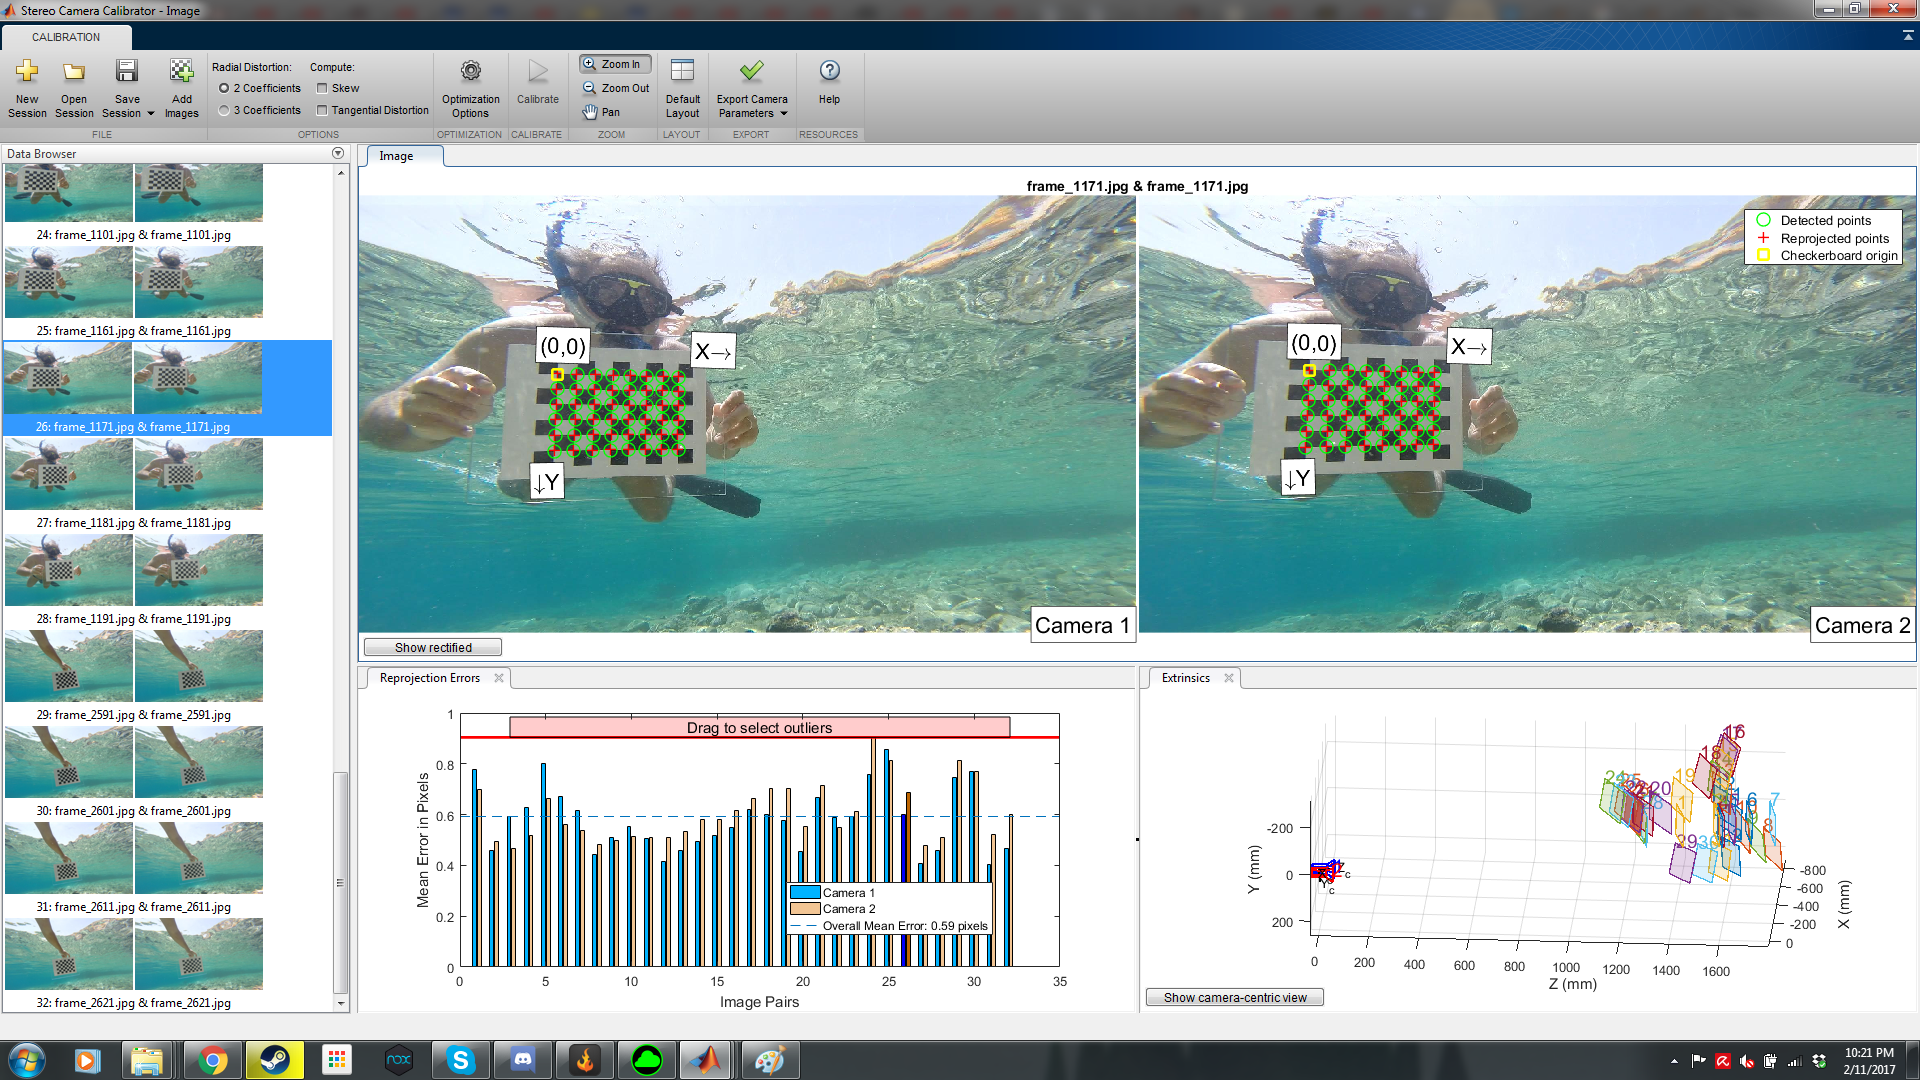
\includegraphics[width=0.95\columnwidth]{./figures/Results_01.png}}
	\caption{MATLAB Stereo Calibrator App GUI.}
	\label{fig:results1}
\end{figure}